% Copyright (c) 2012 Raniere Silva <r.gaia.cs@gmail.com>
% Copyright (c) 2012 Fernando Cezarino <feolce@gmail.com>
% Copyright (c) 2012 Ana Paula Diniz Marques <anapdinizm@gmail.com>
% Copyright (c) 2012 Camile Kunz <camileknz@gmail.com>
% Copyright (c) 2012 Ana Flavia <anaflavia.c.lima@gmail.com>
%
% This file is part of 'MS480 - 2012S2 - Aterro com Obstáculo'.
%
% 'MS480 - 2012S2 - Aterro com Obstáculo' is licensed under the Creative
% Commons Attribution-ShareAlike 3.0 Unported License. To view a copy of
% this license, visit http://creativecommons.org/licenses/by-sa/3.0/.
%
% 'MS480 - 2012S2 - Aterro com Obstáculo' is distributed in the hope
% that it will be useful, but WITHOUT ANY WARRANTY; without even the
% implied warranty of MERCHANTABILITY or FITNESS FOR A PARTICULAR
% PURPOSE.

\section{Distância entre pontos} \label{sse:distance}
Ao utilizar a malha quadriculada, podemos definir a distância entre dois
de seus quadrados de pelo menos três maneiras diferentes:
\begin{enumerate}
    \item $d_l$, que é a menor distência entre qualquer dois pontos dos
        quadrados,
    \item $d_u$, que é a maior distância entre qualquer dois pontos dos
        quadrados, e
    \item $d_c$, que é a distância entre os centros dos quadrados.
\end{enumerate}
Na Figura~\ref{fig:dist_malha} é ilustrado cada uma das distâncias acima
descrita.
\begin{figure}[!htb]
    \centering
    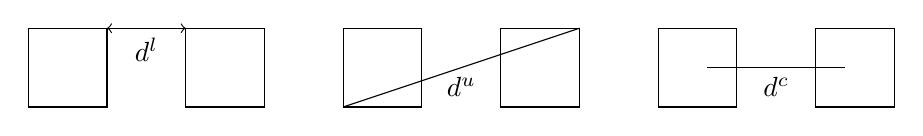
\begin{tikzpicture}
        \draw (0,0) rectangle (1,1);
        \draw (2,0) rectangle (3,1);
        \draw[<->] (1,1) -- (2,1) node[midway, below]{$d^l$};

        \draw (4,0) rectangle (5,1);
        \draw (6,0) rectangle (7,1);
        \draw (4,0) -- (7,1) node[midway, below]{$d^u$};

        \draw (8,0) rectangle (9,1) node[midway](A){};
        \draw (10,0) rectangle (11,1) node[midway](B){};
        \draw (A) -- (B) node[midway, below]{$d^c$};
    \end{tikzpicture}
    \caption{Ilustra\c{c}\~{a}o das dist\^{a}ncias entre quadrados da malha.}
    \label{fig:dist_malha}
\end{figure}
